In this chapter, we explain the necessary background, as well as the related work in the research literature.

\subsection{Background Review}
We discuss the basic background knowledge that helps us throughout the document.

\subsubsection{Convolutional Neural Networks}
First we do a brief introduction for Convolutional Neural Networks (CNN). CNN is a special type of \emph{feed-forward} neural networks, which uses convolution operations to perform the forward computations. They are used in wide range of applications, especially \emph{computer vision}. There are $4$ basic types of layers in a CNN that we would like to mention :
\begin{enumerate}
    \item \textbf{Convolution layer} : uses filters (a.k.a. \emph{kernels}) to detect edges and shapes by convolution with the input map. The filter has certain dimensions and scans the map using certain stride. This helps the network to learn sparse connections and local structures.
    \item \textbf{Pooling layer} : is usually used to reduce the input dimensions through maximizing or averaging using a filter.
    \item \textbf{Upsampling layer} : increases the dimensions of the input map using traditional upsampling methods, such as bilinear upsampling, or learnable upsampling using \emph{deconvolution}.
    \item \textbf{Fully-connected layer} : is a normal feed-forward dense layer, usually used in classification.
\end{enumerate}

\subsubsection{Generative Adversarial Networks}
Generative Adversarial Networks (\emph{GANs}) \cite{goodfellow2014generative} are generative models that can learn through \emph{adversarial training}. GANs have proven to be very good at generating high dimensional data like images. That's why they are used in wide range of applications including image and video generation, image-to-image translation and others.

\begin{figure}[H]
    \centering
    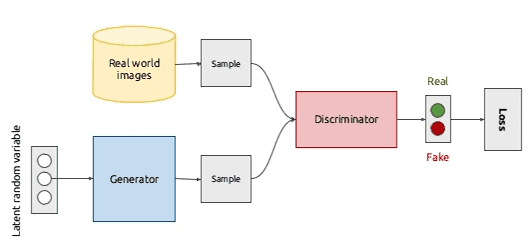
\includegraphics[width=0.8\textwidth]{images/gan-arch.png}
    \caption{The basic architecture of a generative adversarial network (GAN).}
    \label{fig:gan}
\end{figure}

The basic architecture of a GAN (as shown in \ref{fig:gan}) consists of $2$ main networks. A \emph{generator} takes in random noise (usually \emph{latent random variable}) and convert it into a fake data sample. A \emph{discriminator} judges the quality of the fake data sample by distinguishing between real and fake data samples. The discriminator loss (a.k.a. \emph{adversarial loss}) is used to train both generator and discriminator. So, the whole system can be decomposed into a two-player \emph{minimax} formulated as :
\begin{equation}
    min_{G} max_{D} V(D, G) = E_{x \sim Pdata}(x) [log D(x)] + E_{z \sim Pz}(z)[log(1 - D(G(z)))]
\end{equation}

The generator and discriminator networks can be any type of networks. In our case, we use \emph{Convolutional Neural Networks} (CNN), because the output is an image. Consequently, the generator is a CNN that up-samples the latent variable into a complete image. Meanwhile, the discriminator is a classification CNN that encodes the input image and classifies it into real or fake.

The first architecture for a CNN-based GAN goes by the name \texttt{DCGAN} \cite{radford2016unsupervised}. In our work, we focus on a specific type of GANs, named \emph{style-based} (or \emph{latent-based}) GANs.

\subsubsection{Latent Space and Entanglement}
As mentioned before, we focus on a specific type of generative models named \emph{style-based} GANs. These GANs can have artistic control over their outputs, not just sampling data randomly from a prior distribution. The key idea of these models is to use a \emph{latent variable} to control the output, instead of just considering a random noise. This latent variable is sampled from a \emph{latent space} and, then, used to guide the generation process in the generator network using adaptive instance normalization (\emph{AdaIN}).

\emph{AdaIN} is a normalization method that aligns the mean and variance of the content features with those of the style features. It's an extension over \emph{Instance Normalization}, which normalizes the input to a single style specified by the affine parameters. It can be formulated as follows :
\begin{equation}
    AdaIN(x,y) = \sigma(y)(\frac{x - \mu(x)}{\sigma(x)}) + \mu(y)
\end{equation}

The latent space is a made-up space, in which the data is encoded in low dimensional representation. For a good model architecture, the latent space is organized, such that similar features are clustered together and changes in low dimensional latent space maps to similar changes in the generated data. Some the most popular and robust latent-based architectures are \texttt{BigGAN} \cite{brock2019large} and \texttt{StyleGAN} \cite{karras2019stylebased} \cite{karras2020analyzing}. 

\begin{figure}[H]
    \centering
    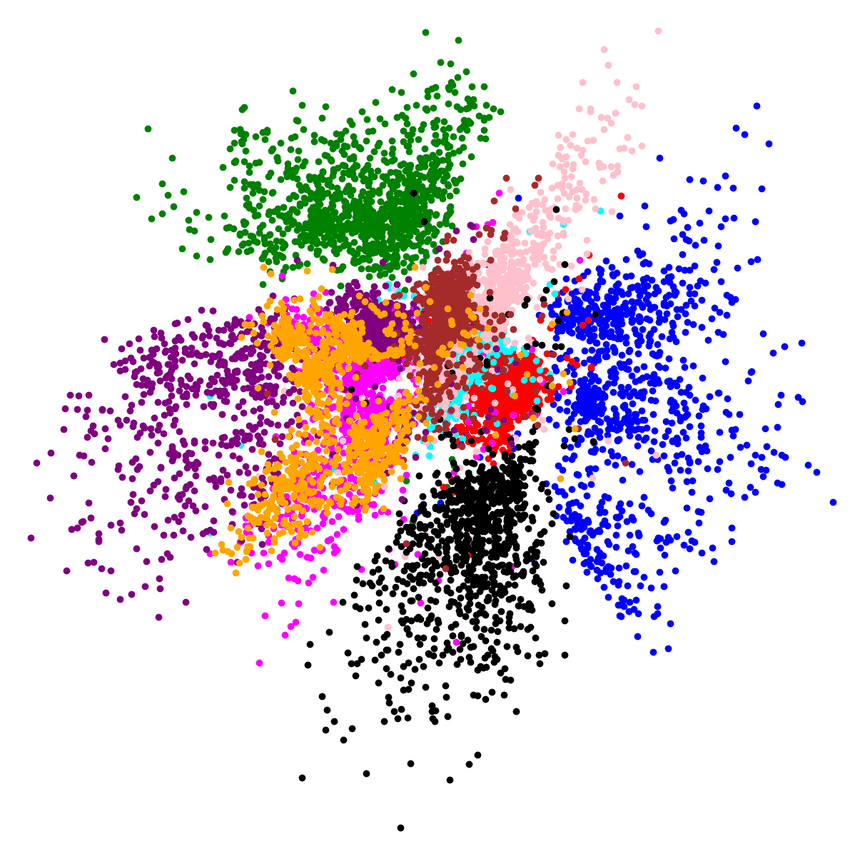
\includegraphics[width=0.6\textwidth]{images/latent-space.png}
    \caption{An example 2D latent space of MNIST digits dataset.}
    \label{fig:lspace}
\end{figure}

Figure \ref{fig:lspace} shows a simple $2D$ latent space for \texttt{MNIST} dataset for digits classification. We can see that we have $10$ clusters corresponding to the $10$ digits. Some clusters are more overlapping than others. It's obvious from the figure that we can learn certain directions to move from one cluster to another in the latent space. However, due to overlapping, certain directions might not be clear or even feasible to obtain. This problem is known as \textbf{entanglement}, which is one of the most important challenges of our work.

The problem of entanglement arises due to the data and training process of the architecture. Some datasets can show heavy correlation between different features, which causes the latent space to be less organized and the features clusters to be overlapping. Thus, the features are entangled in the latent space and extracting independent directions for every feature is hard or even infeasible. Consequently, moving along a certain direction can cause multiple features to change with certain amounts.

\subsubsection{Multi-class Multi-label Text Classification}

\subsection{Face Modelling and Generation}
In this sub-section, an overview is given about face generation and refinement methods.

\subsubsection{Face Generation}
The problem of human face generation is not new to the \emph{AI} research. Many generative models target the problem of face generation from scratch.

\paragraph{StyleGAN}
A new generator architecture is proposed that enables controlling the synthesis of the faces by learning the unsupervised separation of high level features. It generates a complete high quality face image controlled by the latent code. It basically works as follows :
\begin{itemize}
    \item Latent code first is mapped to an intermediate latent space.
    \item The intermediate latent code controls the generator using adaptive instance normalization.
\end{itemize}

\paragraph{Visual Results}
\begin{figure}[H]
    \centering
    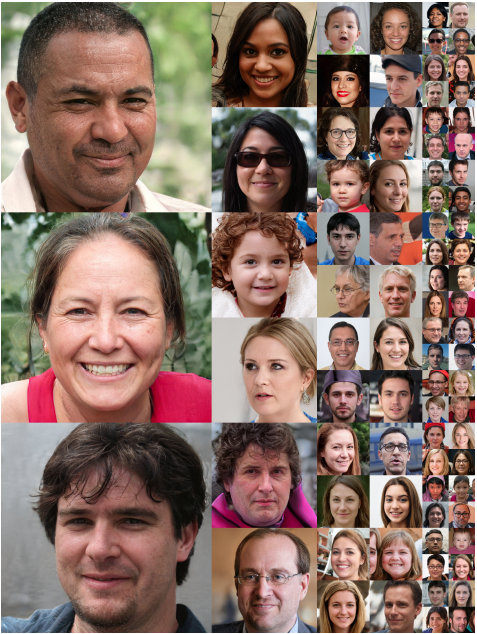
\includegraphics[width=0.6\textwidth]{images/stylegan-results.png}
    \caption{Visual results of StyleGAN2.}
    \label{fig:stgan_res}
\end{figure}

Figure \ref{fig:stgan_res} shows visual result samples from \texttt{StyleGAN2}, which is the revisited version of \texttt{StyleGAN}.

\paragraph{StyleGAN latent manipulation}
Subsequent research work follows \texttt{StyleGAN} to try latent manipulation for more control over the generated faces. These methods include \texttt{Image2StyleGAN} \cite{abdal2019image2stylegan}, \texttt{Image2StyleGAN++} \cite{abdal2020image2stylegan}, \texttt{InterfaceGAN} \cite{shen2020interfacegan}, \texttt{StyleRig} \cite{tewari2020stylerig} and \texttt{StyleFlow} \cite{abdal2020styleflow}. All of these work targeted the directed manipulation of \emph{StyleGAN} latent space to change certain facial features. However, none of these methods target complete generation of new face from bare description, which is, also, known as \emph{conditioned sampling}. 

On the other hand, our work target face generation from bare description. Consequently, we utilize the concept of directed manipulation to do conditioned sampling, which is described later in this document.

\paragraph{Faces à la Carte}
To our knowledge, this \cite{wang2020faces} is the only current open-source research work that addressed the problem of face generation from text. It's based on \texttt{StyleGAN2} and uses a general framework to extract the feature directions and reach the target face.

We couldn't replicate their results, because the authors don't provide sufficient information about their method. However, we managed to gain some insights that helped us throughout the project.

\begin{figure}[H]
    \centering
    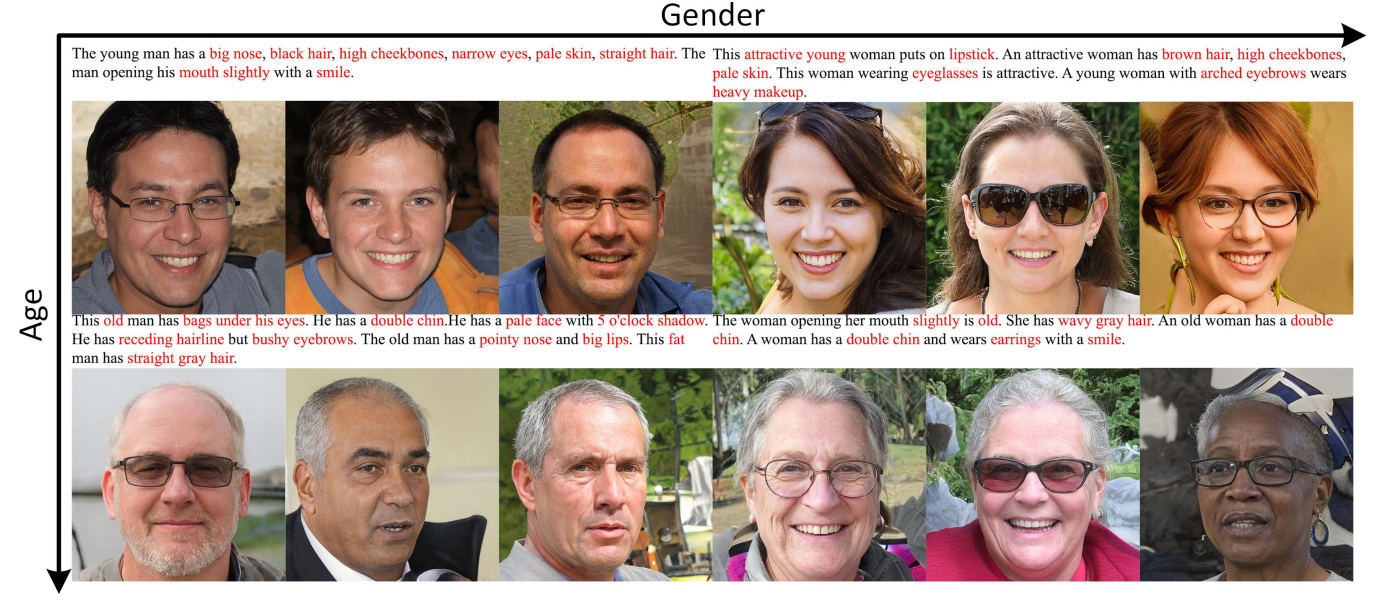
\includegraphics[width=\textwidth]{images/face-carte.png}
    \caption{Visual results of Faces à la Carte.}
    \label{fig:face_carte}
\end{figure}

Figure \ref{fig:face_carte} shows the visual results that the authors included in their paper. While being conservative about some of their work, we still consider this as the only former open-source research work related to our problem.

\paragraph{NVAE}
The paper \textbf{NVAE: A Deep Hierarchical Variational Autoencoder} \cite{vahdat2021nvae} is a recent research work that discusses the usage of Variational Autoencoder (\emph{VAE}) to generate high quality image controlled by a latent variable. It uses normalizing flows to control the output features. \emph{Normalizing flows} is a method of mapping an unknown distribution to a known distribution (normal or uniform). It's basically used to generate complex distributions from simple normal distributions.

\begin{figure}[H]
    \centering
    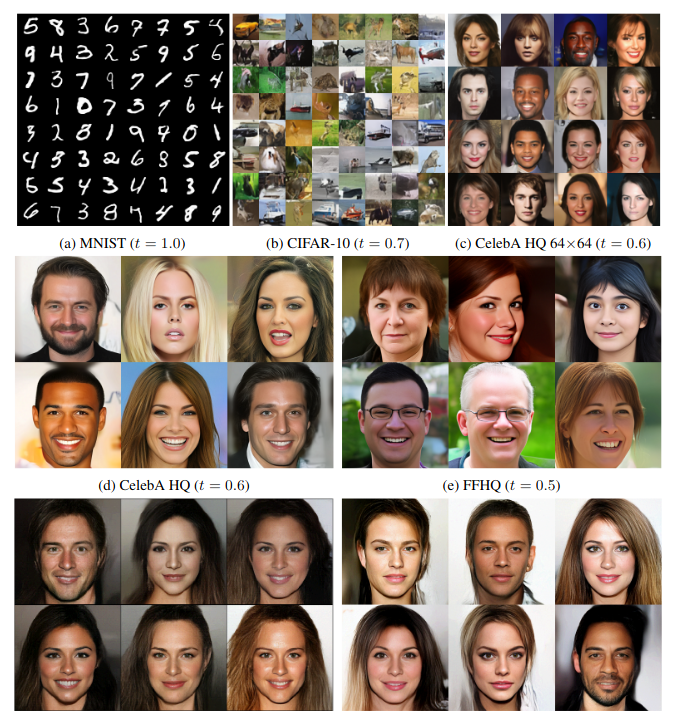
\includegraphics[width=0.8\textwidth]{images/nvae.png}
    \caption{Visual results of NVAE.}
    \label{fig:nvae}
\end{figure}

\subsubsection{Face Refinement}
The process of face generation can be inaccurate, thus the stage of face refinement is a must, in order to be able to independently edit some of the facial features.

\paragraph{AttGAN}
\texttt{AttGAN} \cite{he2018attgan} uses an encoder-decoder architecture for the generator, where the decoder takes an attribute vector telling it which attributes are existing and which are not. There’s a classifier after the decoder to get the attribute vector of the output image. The decoder is trained to get the same input image if the attribute vector was the input attribute vector and to get an output image with a new attribute vector which makes the classifier get the same attribute vector if the output image was given to it. The architecture is shown in figure \ref{fig:attgan}, meanwhile the results are shown in figure \ref{fig:attgan_res}

\begin{figure}[H]
    \centering
    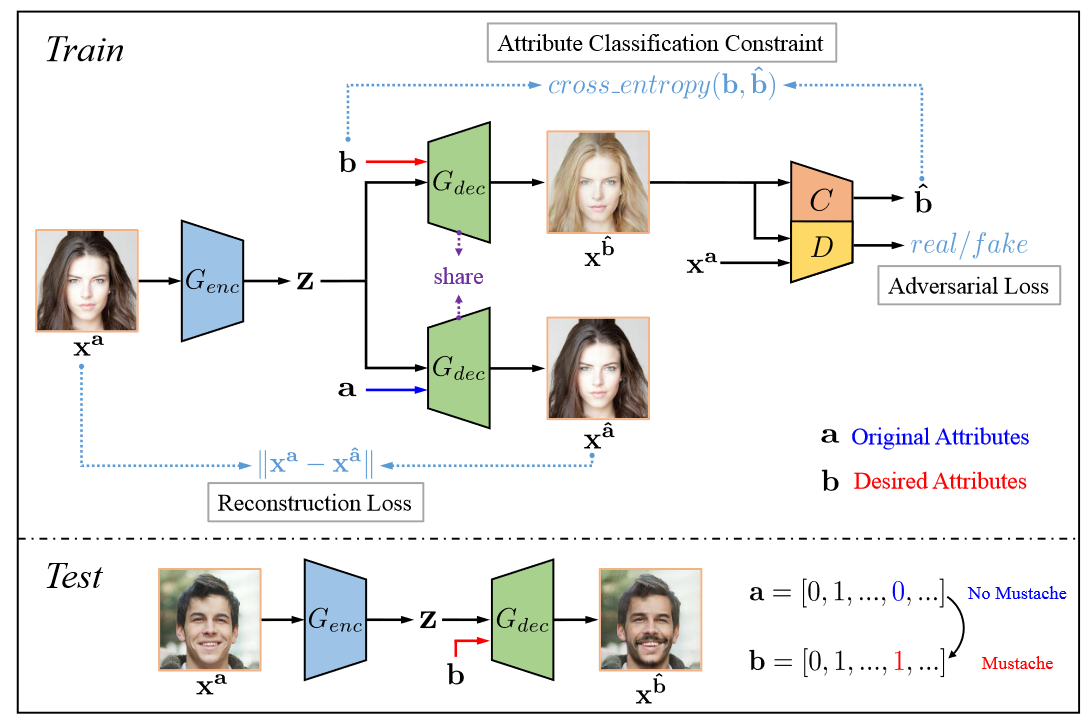
\includegraphics[width=0.8\textwidth]{images/attgan.png}
    \caption{Complete architecture of AttGAN.}
    \label{fig:attgan}
\end{figure}

\begin{figure}[H]
    \centering
    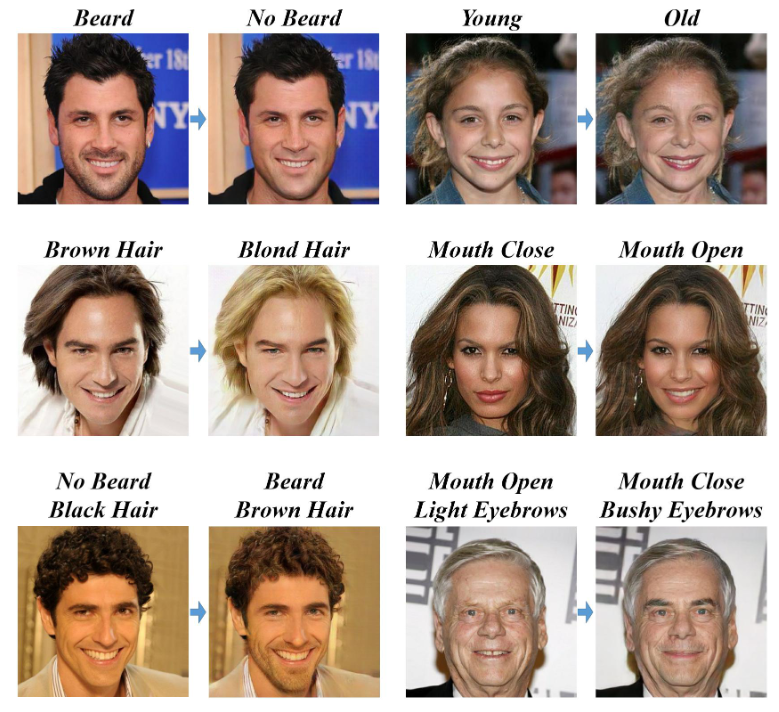
\includegraphics[width=0.8\textwidth]{images/attgan-results.png}
    \caption{Visual results of AttGAN.}
    \label{fig:attgan_res}
\end{figure}

\paragraph{InjectionGAN}
\texttt{InjectionGAN} \cite{9119402} uses the same concepts as AttGAN, but it has one more concept, which is using Feature-wise Linear Modulation (FiLM) layer which successfully infers information from external data and applies it as an affine transformation parameter to vision tasks, so they propose a new type of skip connection layers between encoder and decoder of the generator to add the new attributes shown in figure \ref{fig:injgan}. Visual results of InjectionGAN are shown in figure \ref{fig:injgan_res}

\begin{figure}[H]
    \centering
    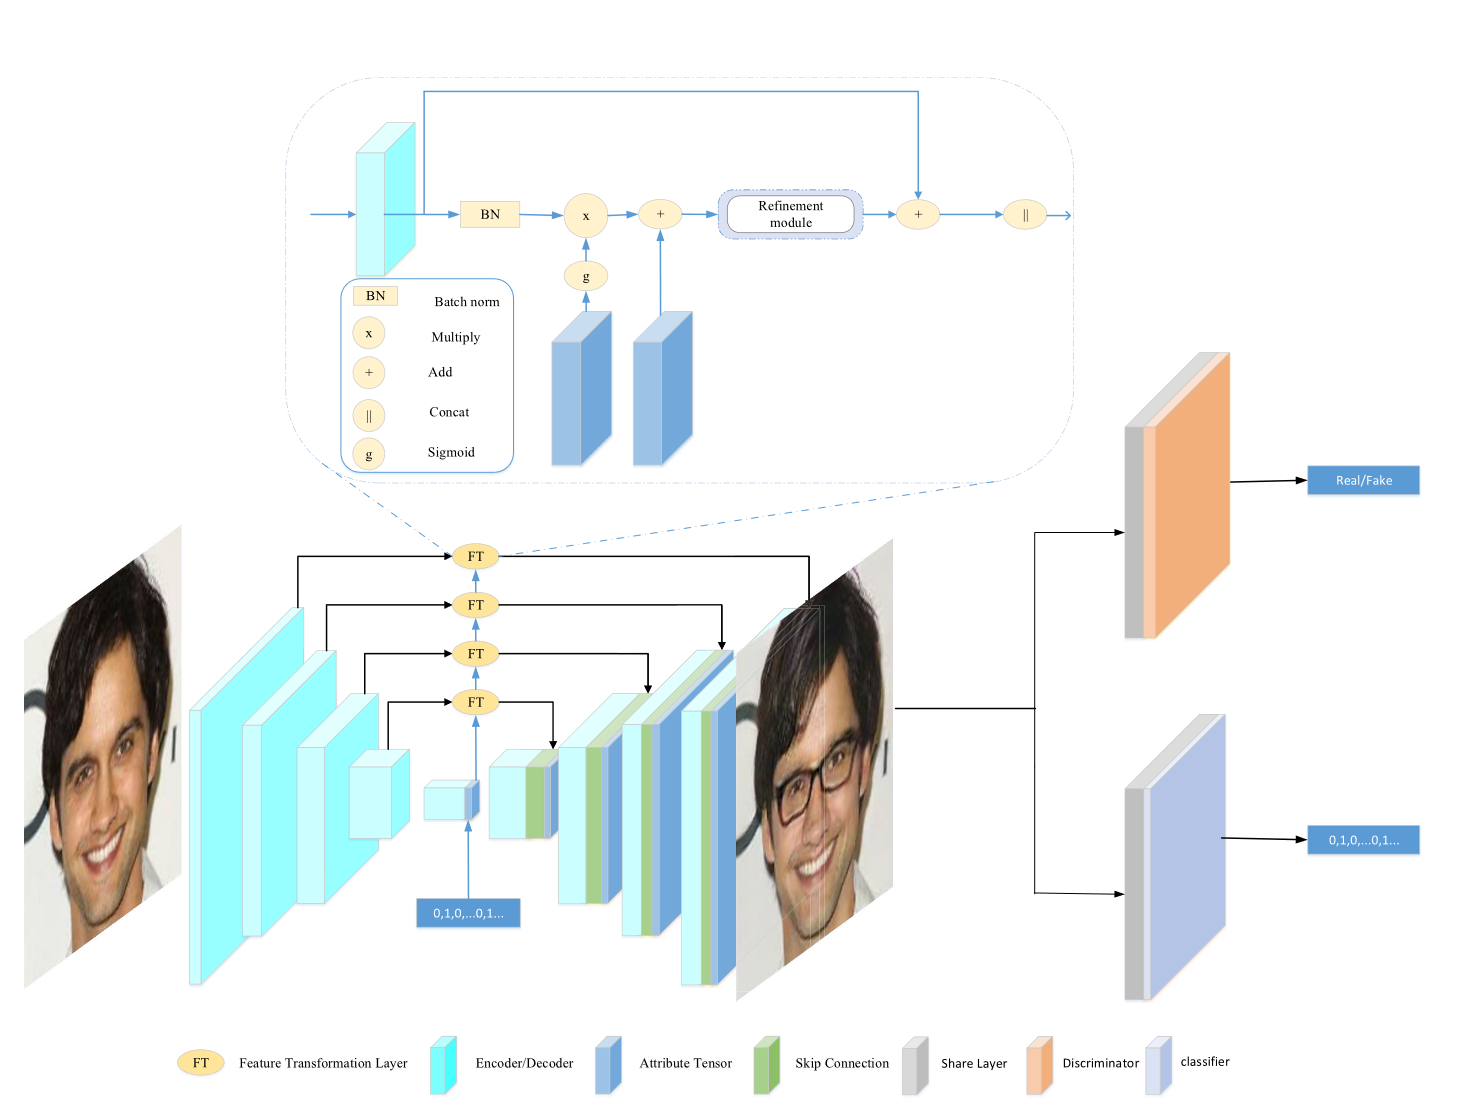
\includegraphics[width=0.8\textwidth]{images/injectiongan.png}
    \caption{Complete architecture of InjectionGAN.}
    \label{fig:injgan}
\end{figure}

\begin{figure}[H]
    \centering
    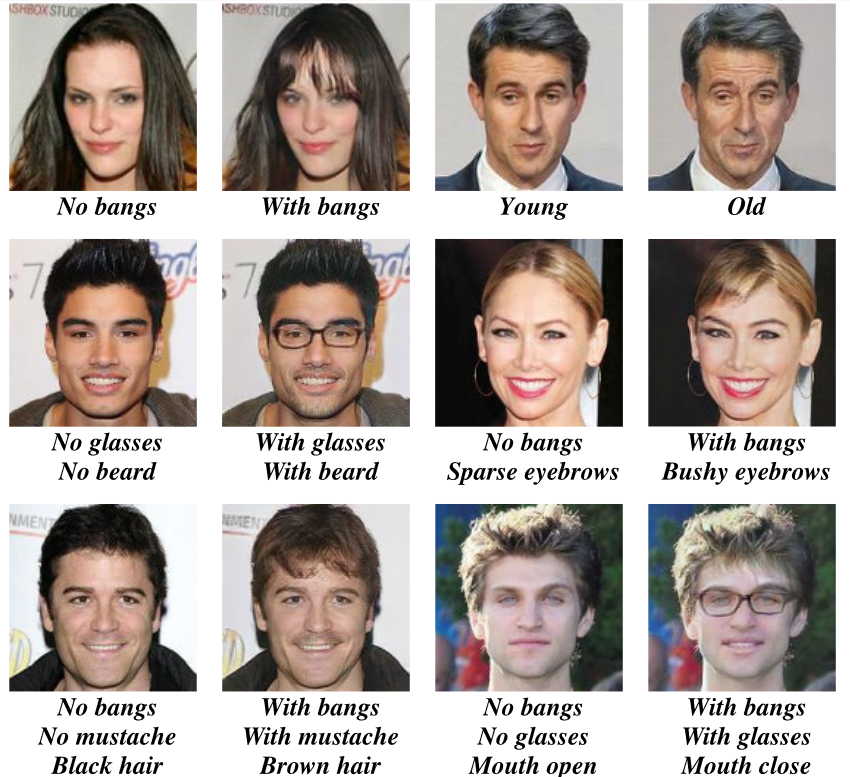
\includegraphics[width=0.8\textwidth]{images/injectiongan-results.png}
    \caption{Visual results of InjectionGAN.}
    \label{fig:injgan_res}
\end{figure}

\paragraph{Facelet-Bank for Fast Portrait Manipulation}
\texttt{Facelet Bank} \cite{chen2018faceletbank} follows the idea of navigation in GANs latent space, they added a new module called Facelet bank. It’s used as skip connections. It takes a bottleneck output from the decoder as input and passing it to a block of CNN layers and add it to the bottleneck output. This summation does the operation of the navigation in the latent space, so the Facelet layer should be trained to get the correct added value to different bottleneck outputs to  the same face with changing a specific attribute. Figure \ref{fig:facelet} shows the complete architecture, while figure \ref{fig:facelet_res} shows the visual results.

\begin{figure}[H]
    \centering
    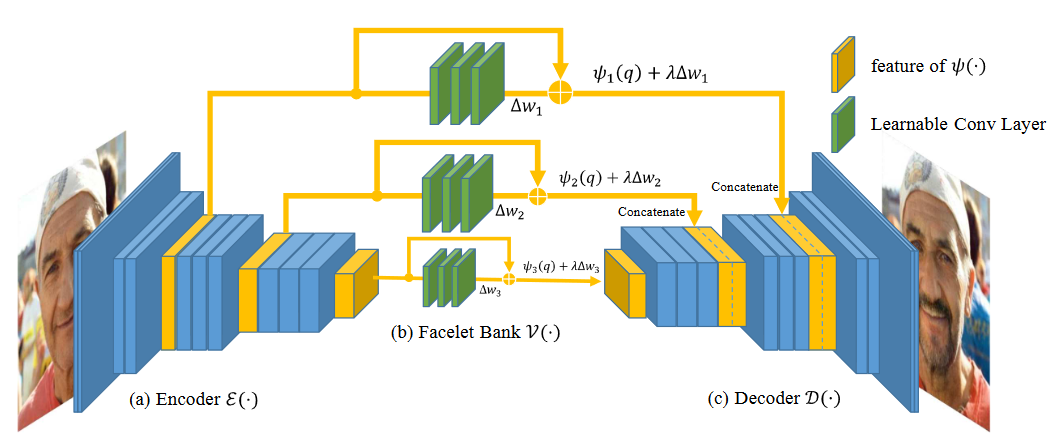
\includegraphics[width=0.8\textwidth]{images/facelet.png}
    \caption{Complete architecture of Facelet Bank.}
    \label{fig:facelet}
\end{figure}

\begin{figure}[H]
    \centering
    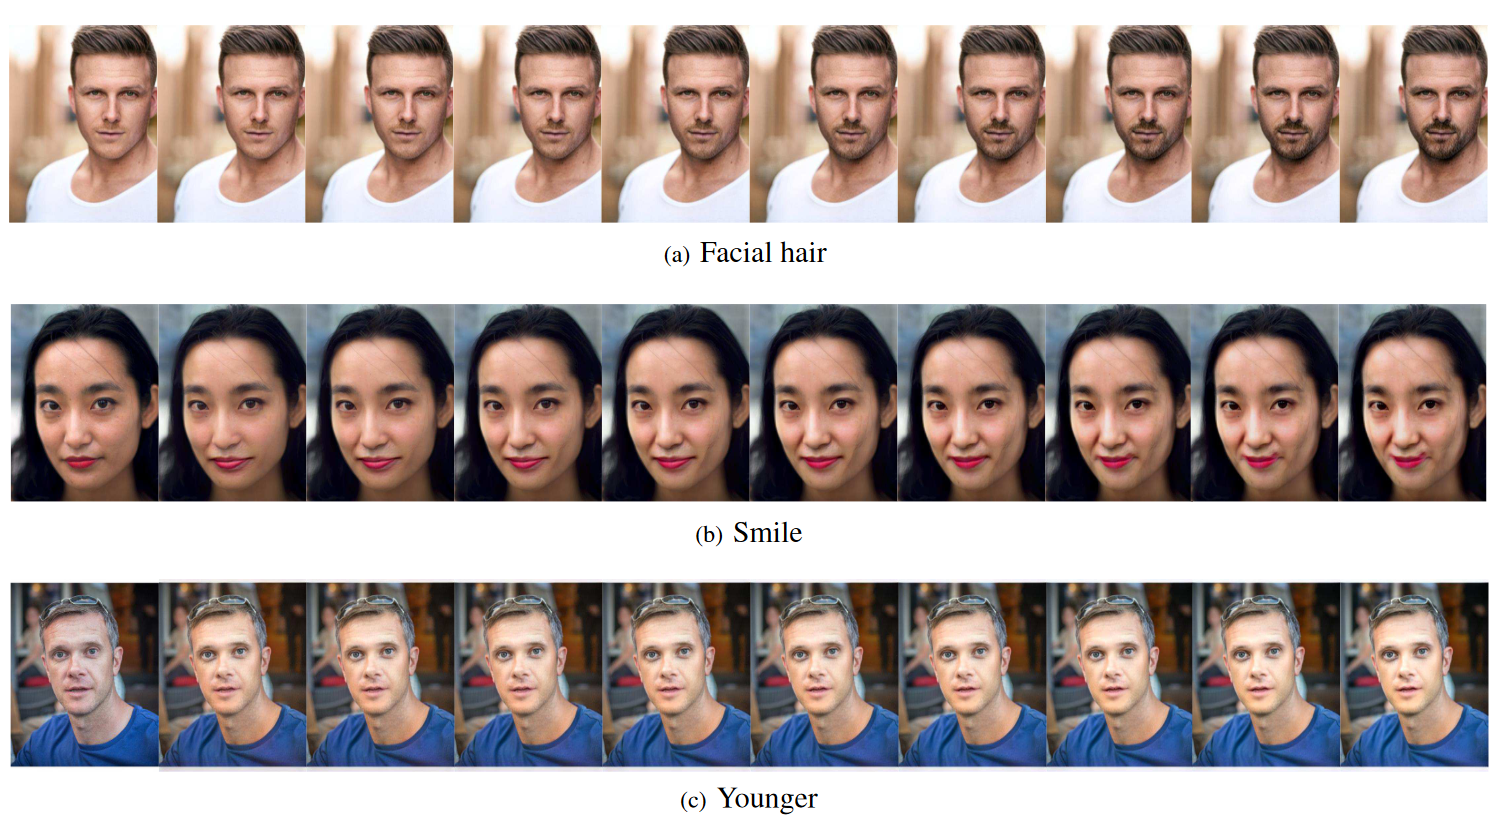
\includegraphics[width=0.8\textwidth]{images/facelet-results.png}
    \caption{Visual results of Facelet Bank.}
    \label{fig:facelet_res}
\end{figure}

\subsection{Face Rotation}
In this sub-section, we discuss different methods and approaches to generate multiple head poses from a single image. Note that, we focus on the methods that rotate a face, provided by a single image, with multiple angles of rotation, not just head frontalization. Also, the methods are ordered according to priority based on \emph{performance}, \emph{visual results} and \emph{involved work}.

\subsubsection{Rotate-and-Render}

\paragraph{Brief Description}
A DNN-based method under the title of \textbf{Rotate-and-Render: Unsupervised Photorealistic Face Rotation from Single-View Images} \cite{zhou2020rotateandrender}. The network is based on \emph{3D face modelling} with \emph{unsupervised deep learning}. 

\paragraph{Workflow}
It consists of three stages : 
\begin{itemize}
    \item \textbf{3D face fitting} which generates a 3D model of the face and extracts the face texture.
    \item \textbf{Rotate-and-render} which rotates the face in 3D space and renders it in different poses.
    \item \textbf{Render-to-image} which projects the 3D render of the face into a 2D image.
\end{itemize}
\textbf{Note :} The architecture, also, ensures \emph{cycle-consistency} through re-projecting the face into the initial pose.

\paragraph{Visual Results}
\begin{figure}[H]
    \centering
    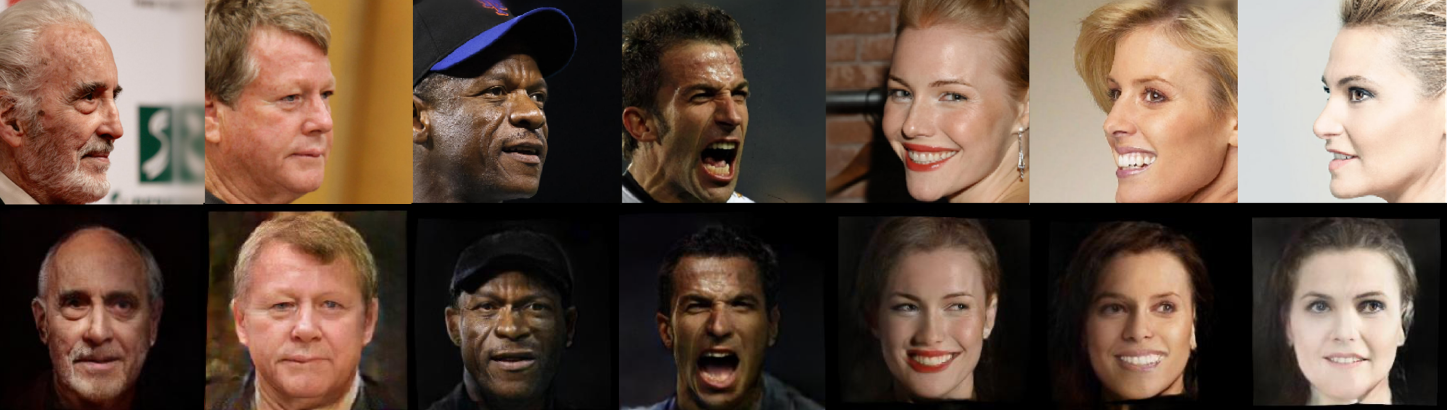
\includegraphics[width=\textwidth]{images/rotate-and-render.png}
    \caption{Visual results of Rotate-and-render network.}
    \label{fig:r&r}
\end{figure}

\subsubsection{DepthNets}

\paragraph{Brief Description}
A DNN-based method under the title of \textbf{Unsupervised Depth Estimation, 3D Face Rotation and Replacement} \cite{moniz2018unsupervised}. The network is based on \emph{casting} a specific face to a pose provided by another face in an \emph{unsupervised way}.

\paragraph{Workflow}
It consists of three stages :
\begin{itemize}
    \item \textbf{Landmark extraction} from both faces.
    \item \textbf{Image-to-image translation}.
    \item \textbf{Siamese-like architecture} that compares the generated face with the original one.
\end{itemize}

\paragraph{Visual Results}
\begin{figure}[H]
    \centering
    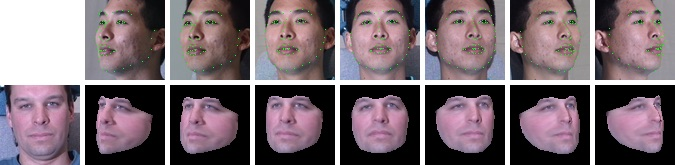
\includegraphics[width=\textwidth]{images/depthnets.png}
    \caption{Visual results of DepthNets.}
    \label{fig:dn}
\end{figure}

\subsubsection{PosIX-GAN}

\paragraph{Brief Description}
A DNN-based method under the title of \textbf{PosIX-GAN: Generating multiple poses using GAN for Pose-Invariant Face Recognition} \cite{inbook}. The network generates the provided faces in \emph{9 angles of rotation} in an \emph{end-to-end manner} that relies on datasets to train GANs.

\paragraph{Workflow}
It's an end-to-end network that depends on datasets for training.

\paragraph{Visual Results}
\begin{figure}[H]
    \centering
    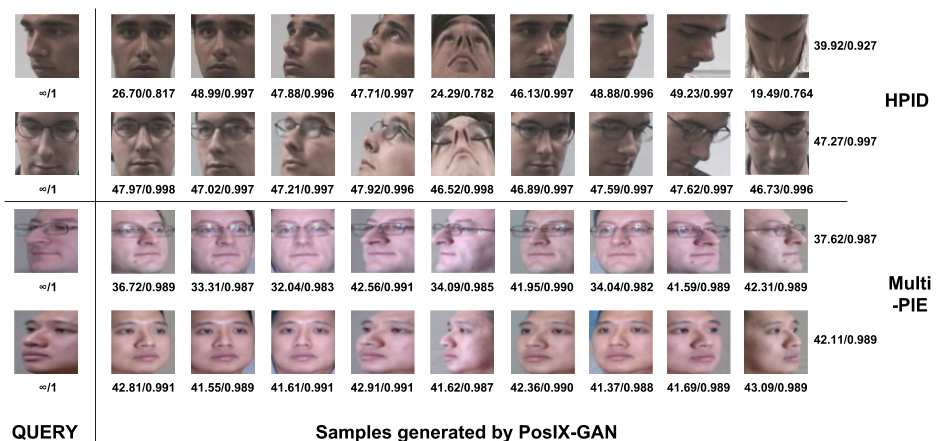
\includegraphics[width=0.8\textwidth]{images/posix-gan.png}
    \caption{Visual results of PosIX-GAN.}
    \label{fig:posix}
\end{figure}

\subsubsection{CAPG-GAN}

\paragraph{Brief Description}
A DNN-based method under the title of \textbf{Pose-Guided Photorealistic Face Rotation} \cite{8578974}. The network generates different head poses using a \emph{pose-conditioned generator} and \emph{couple-agent discriminator} that discriminates both identity and pose.

\paragraph{Workflow}
It's an end-to-end network that depends on datasets for training.

\paragraph{Visual Results}
\begin{figure}[H]
    \centering
    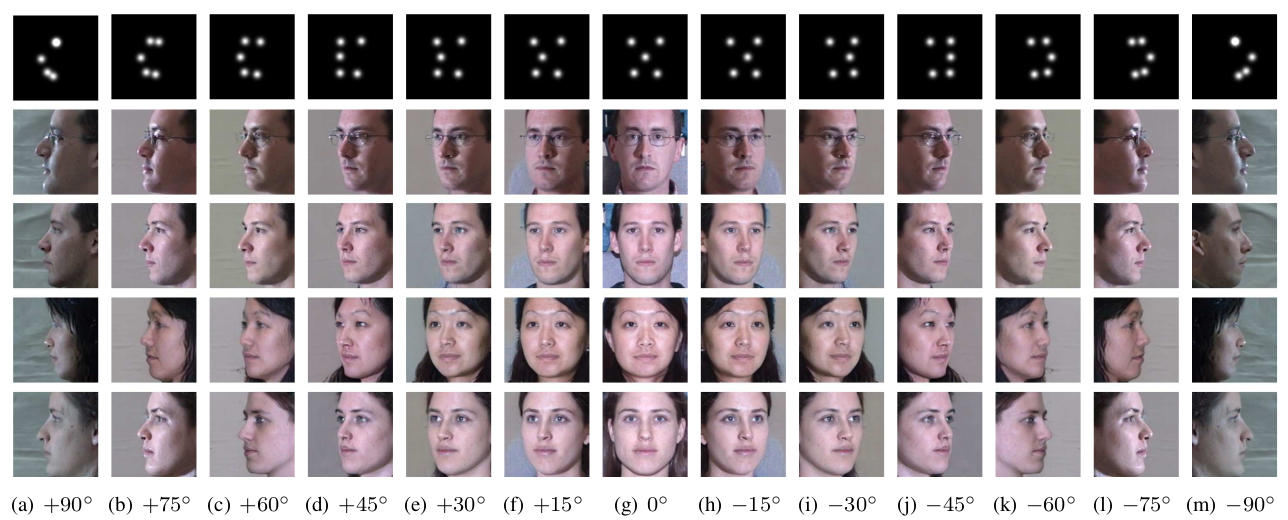
\includegraphics[width=\textwidth]{images/capg-gan.png}
    \caption{Visual results of CAPG-GAN.}
    \label{fig:capg}
\end{figure}

\subsection{Comparative Study of Previous Work}
From our previous discussion, we can see that \texttt{StyleGAN2} offers the best quality of faces, while being very flexible. The architecture is used in various research works related to image generation. Other approaches don't have the same flexibility and robustness. That's why we opted to use \texttt{StyleGAN2} as our main generative model. 

\texttt{Faces à la Carte} paper does not provide enough details about their method, as well. This is one of the reasons that encourages us to work on this project, in order to provide are clear pipeline for the problem solution.

Regarding face refinement, the most promising method is \texttt{Facelet Bank}, which can be used on high quality image. Also, the \emph{facelet bank} module is flexible enough to handle multiple facial features. However, in our final system, we chose not to go with this architecture for reasons, mentioned later in the document.

Finally, for face rotation, \texttt{Rotate-and-Render} and \texttt{DepthNets} offer an unsupervised framework for multiple face poses generation. This is better and much easier to adapt than other supervised methods, mainly because most of head poses datasets are not open-source. \texttt{Rotate-and-Render} can produce better visual results than \texttt{DepthNets}, because it can account for features such as hair through \emph{image inpainting} using \emph{image-to-image translation}. Overall, this yields better visual results.

\subsection{Implemented Approach}
Our system implements $3$ main functionalities, which are \textbf{text-to-face generation} (input can be \emph{speech} or \emph{text}), \textbf{face refinement} and \textbf{multiple head poses generation}. After extensive research and experimentation, we come up with our working pipeline that achieves our project goal.

\subsubsection{Face Generation from Description}
First of all, we start with our core and the most innovative part of our project. Face generation from bare description is very popular problem, yet few research works target it. To our knowledge, \texttt{Faces à la Carte} is the only available research paper that targets this problem. As we mentioned, the authors does not offer enough details about their method. Consequently, we have to utilize the related work to carefully design a fast and robust system for such problem. 
Our system can take different kinds of descriptions, including audio, text and manual inputs. That's why we have to create multiple stages of input processing and not to use direct end-to-end networks. 

The first processing stage is \emph{speech recognition}, which translates the speech into textual description. We opt to use \texttt{DeepSpeech2} \cite{amodei2015deep}, which is one of the most popular speech recognition architectures.

The second processing stage is \emph{text processing}, which converts the textual description into numerical attributes values. For this stage, we have many options, including classical and DL-based methods. However, we choose to work with \texttt{DistilBERT} \cite{sanh2020distilbert} due to multiple reasons. Basically, \texttt{DistilBERT} is a lightweight architecture that does not have a very big memory footprint. It's fast and easily tuned to our needs. Moreover, it does not use \emph{recurrent neural networks}, which are slow at inference time. Finally, we can adapt it to our desired output, which is not just classification, but the actual numerical values of the facial features.

The third and last processing stage is \emph{code generation}, which transforms the numerical attributes values into a face embedding that is used to guide the face generation process. This stage is completely designed from scratch and refined, iteratively, with face generative model (\texttt{StyleGAN2}). However, some previous research works are used for guidance, especially \texttt{Image2StyleGAN}, which guided our feature directions extraction process. However, our system considers more facial features than any of the previous works.

Finally, we come to the actual face generation model. For this, we opt to use \texttt{StyleGAN2}. The reason behind this choice is that \texttt{StyleGAN2} is the one of the most powerful image generators that produce high quality images. It's very flexible and can be adapted to many applications. Moreover, it does not required special hardware to be tuned, which is the case in \texttt{BigGAN} that requires \emph{Tensor Processing Units} (\emph{TPUs}).

\subsubsection{Face Refinement}
For the face refinement module, we choose to adapt our work in \textbf{face generation} to be used for refinement as well. This is mainly done to avoid including another model, which would have increased the memory footprint. Moreover, latent manipulation of \texttt{StyleGAN2} can offer better results than most face refinement architectures with more facial features to include. Consequently, \texttt{StyleGAN2} latent manipulation is considered for face refinement with an extended set of facial attributes to refine.

\subsubsection{Multiple Head Poses Generation}
Although it's possible to extract feature directions for the generated head poses for \texttt{StyleGAN2} as well, we don't consider using it for face rotation. This is mainly because face pose directions suffer from heavy entanglement with other features. Moreover, these directions don't preserve the face identity and can cause serious illumination problems. Consequently, we only keep this method as a backup plan. However, \texttt{Rotate-and-Render} is our main multiple head pose generation method. We used the same workflow to create our face rotation pipeline and integrate it to our system. The main reason behind choosing \texttt{Rotate-and-Render} is that the whole workflow can be decomposed into separate modules to can be edited and implemented to fit our needs. Also, it is an unsupervised architecture, which makes it easy to work with. Finally, it offers decent results compared to other architectures.
